\section{问题三的滚动调整模型}

\subsection{光伏预报对齐与修正}

在发布时刻 $\tau\in\{0,6,12,18\}$，将未来各小时光伏预报作为该小时 6 个区间的常值。对每个提前期，使用此前 14 日同一发布时刻的预报误差中位数进行偏差修正。负载预测沿用问题二的方法，并以当天已经观测到的最近 18 个区间误差中位数修正未来负载。上述修正都只依赖发布时刻以前的信息。

\subsection{相对上一版计划的再优化}

记调整前有效计划为 $x_t^{\rm old}$，新计划为 $x_t^{\rm new}$，引入
\begin{equation}
x_t^{\rm new}-x_t^{\rm old}=a_t^+-a_t^-,\qquad a_t^+,a_t^-\geq0.
\end{equation}
对尚未执行区间，调整增量费用为
\begin{equation}
\Delta C_{\tau}=\sum_{t\geq\tau}p_t\left(1.5a_t^+-0.5a_t^-\right).
\label{eq:adjust}
\end{equation}
其中 $-0.5p_ta_t^-$ 表示取消原计划后退回一半费用，另一半作为违约成本保留。每次再优化固定所有已执行区间，只更新未来计划；最终费用为
\begin{equation}
C_3=\sum_t p_tx_t^{(0)}+\sum_{\tau\in\{6,12,18\}}\Delta C_{\tau}
+5\sum_t p_tu_t.
\end{equation}

\subsection{四次预报方案结果}

使用全部四次预报时，初始计划费、净调整费用和紧急购电费分别为
$1359.75$ 万元、$85.15$ 万元和 $28.31$ 万元，总费用为 $1473.21$ 万元。
与问题二相比，总费用下降 $34.92$ 万元，紧急购电量从 $27.80$ 万
$\mathrm{kWh}$ 降至 $5.38$ 万 $\mathrm{kWh}$，说明日内预报显著降低了供电缺口。

\subsection{更新时刻消融}

为判断每次预报是否值得采用，依次比较 $S_0=\{0\}$、
$S_1=\{0,6\}$、$S_2=\{0,6,12\}$、$S_3=\{0,6,12,18\}$。结果见表~\ref{tab:ablation}。

\begin{table}[H]
\centering
\caption{不同预报更新集合的全年成本与紧急购电}
\label{tab:ablation}
\begin{tabular}{lrrr}
\toprule
策略 & 总费用/万元 & 紧急购电/kWh & 净调整费用/万元 \\
\midrule
$S_0$ & 1520.73 & 259807.05 & 0.00 \\
$S_1$ & 1464.58 & 89932.77 & 48.32 \\
$S_2$ & 1465.88 & 60791.05 & 71.54 \\
$S_3$ & 1473.21 & 53828.47 & 85.15 \\
\bottomrule
\end{tabular}
\end{table}

6:00 更新使总费用下降 $56.15$ 万元，是必要更新；加入 12:00 后虽然少购约
$2.91$ 万 $\mathrm{kWh}$ 紧急电量，但总费用反而增加 $1.30$ 万元；再加入
18:00 又增加 $7.33$ 万元。因此，在当前结算规则和预测质量下，推荐只在 6:00
进行一次日内调整。12:00 和 18:00 预报具有运行安全价值，但不具有净经济价值。

\begin{figure}[H]
  \centering
  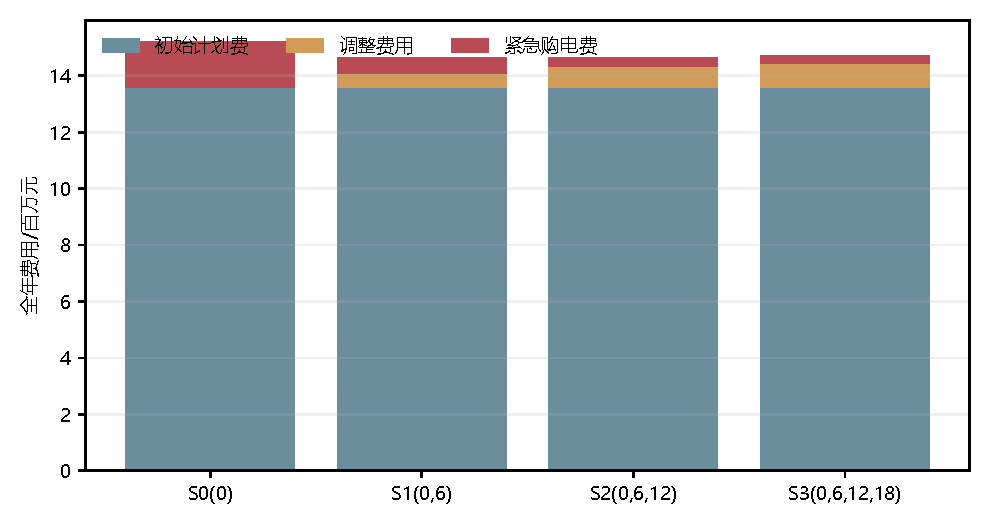
\includegraphics[width=0.86\textwidth]{../figures/p3_update_ablation.pdf}
  \caption{预报更新时刻消融的费用分解}
  \label{fig:p3ablation}
\end{figure}
